% header.tex - DESC
% Iago Mosqueira - JRC. 2012
%

%% gets rid of navigation symbols
\setbeamertemplate{navigation symbols}{}

%% colors
\definecolor{ecblue}{RGB}{1,70,147}
\definecolor{jrcblue}{RGB}{55,172,222}

\setbeamercolor{normal text}{fg=black,bg=white}
\setbeamercolor{structure}{fg=ecblue} 

%% Images
% footer image
\pgfdeclareimage[height=5.5mm]{footimage}{tex/footer}

% header image
\pgfdeclareimage[width=0.1575\paperwidth]{headimage}{tex/header}

% title page image
\pgfdeclareimage[width=0.6\textwidth]{titlegraphic}{graphics/front}

%% footline
%% left: date as in title
\newcommand{\footlinetext}{\insertdate}
\setbeamertemplate{footline}{
\begin{minipage}{58mm}
\hspace{7.5mm} \footlinetext
\end{minipage}
\hspace{0.1mm}
%% center: jrc logo
\begin{minipage}{8.5mm}
 \pgfuseimage{footimage}
\end{minipage}
\hspace{0.1mm}
%% right: page number
\begin{minipage}{50mm}
 \flushright \insertframenumber
\end{minipage}
}


%% headline
\setbeamercolor{shadedhead}{bg=jrcblue}
\setbeamertemplate{headline}{
\leavevmode\hbox{%
%% uniform box
\begin{beamercolorbox}[wd=\textwidth,ht=0.1447\paperheight,dp=0ex]{shadedhead}%
	%% EC logo
	\centering
	%% 0.02895
  \vspace{-0.044\paperheight}
	\pgfuseimage{headimage}
\end{beamercolorbox}%
}}

%% title page
\setbeamertemplate{title page}{

% title
\vspace{6ex}
\centering
{\fontsize{18}{22}\selectfont
\bfseries
\color{ecblue}\inserttitle}
\vspace{6ex}

% title graphic
\begin{columns}[Tc]
\column{0.5\textwidth}
%\pgfuseimage{titlegraphic}
	\vskip-1cm
  \hskip-2.5cm % or \vspace{-2cm} 
  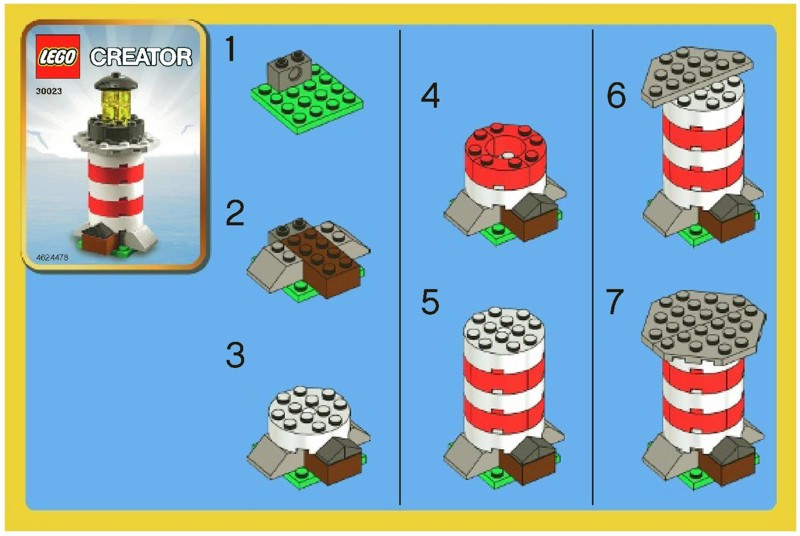
\includegraphics[width=1.5\textwidth]{graphics/front.jpg}

\column{0.4\textwidth}
% author

\insertauthor
\end{columns}

% subtitle
\insertsubtitle


% affiliation
\insertinstitute
}

%% frame title
\setbeamertemplate{frametitle}
{
\color{jrcblue}\vspace{2ex}\fontsize{12}{16}\selectfont
\textbf{\insertframetitle}
\par
}


% bullet points
\setbeamertemplate{itemize items}[circle] % if you want a ball
\setbeamertemplate{itemize subitem}[circle] % if you wnat a circle
\setbeamertemplate{itemize subsubitem}[circle] % if you want a triangle
